\section{The URDAD analysis and design process}

In this section we will introduce URDAD from the perspective of a quality driven process generating an analysis and design model which enforces certain model and process qualities.  URDAD\cite{solms_generating_2009} provides a service oriented analysis and design methodology, a metamodel introducing the semantics (modeling constructs) for an URDAD based domain specific language (the \emph{URDAD-DSL}), as well as a concrete text grammar which can be used to populate an URDAD model complying to the metamodel. A graphical grammar and diagram-based tooling around that grammar are under development. 

Services are recursively assembled from lower level services with leaf services representing services which are sourced from the environment. These may include persistence services, services sourced from the execution frameworks or implementation languages, services sourced from off the external systems as well as manually executed services provided by business partners, business units, and so on.

%-----------------------------------------------------------

\subsection{Quality drivers employed by URDAD}

The model and process quality drivers discussed in \ref{sec:modelQualityDriversAndMetrics} are built into the URDAD process. Table \ref{tab:qualityDrivers} lists the employed model quality drivers and the model qualities they are meant to support.

\begin{table}[h]
 \caption{URDAD model quality drivers related to model qualities.}
 \label{tab:qualityDrivers}
\begin{tabular}{|l|cc|cccccccc|} \hline
\multirow{4}{*}{\bf Quality-driver} & \multicolumn{10}{c|}{\bf Model qualities} \\ \cline{2-11}
& & & \multicolumn{8}{c|}{Pragmatic model qualities}\\ \cline{4-11}
    & \begin{sideways}Semantic\end{sideways} & \begin{sideways}Syntactic\end{sideways}  & \begin{sideways}Simplicity\end{sideways}
    & \begin{sideways}Completeness\end{sideways} & \begin{sideways}Modifiability\end{sideways} & \begin{sideways}Consistency\end{sideways}
    & \begin{sideways}Decoupling\end{sideways} & \begin{sideways}Cohesion\end{sideways} & \begin{sideways}Reusability\end{sideways}
    & \begin{sideways}Traceability\end{sideways} \\ \hline
%                                       Semantic     Syntax        Simplicity  Completeness   Modifiable  Consistent  Decoupled    Cohesion     Reuse        Traceable
Define metamodel or ontology                   & \checkmark & \checkmark & \checkmark & \checkmark & \checkmark & \checkmark & \checkmark &            &            & \checkmark \\
Define concrete DSL grammars                   &            & \checkmark & \checkmark &            & \checkmark &            &            &            &            
& \\
Fix levels of granularity                      &            &            & \checkmark &            & \checkmark &            &            &            &
\checkmark & \checkmark \\ 
Decouple services via contracts                &            &            & \checkmark &            & \checkmark &            & \checkmark &            & \checkmark & \checkmark \\ 
Apply single reponsibility principle           &            &            & \checkmark &            & \checkmark &            &            & \checkmark & \checkmark & \checkmark \\ 
Specify testable pre- \& post-conditions       &            &            &            & \checkmark & \checkmark & \checkmark &            &            &            &  \\ 
Localize process within controller             &            &            & \checkmark &            & \checkmark &            & \checkmark & \checkmark & \checkmark & \checkmark \\ 
Include traceability Links                     &            &            & \checkmark & \checkmark & \checkmark & \checkmark &            &            &            & \checkmark \\ \hline 
\end{tabular}
  
\end{table}

In particular, we have defined a metamodel for URDAD which has been transformed into an ontology with URDAD model validated against the metamodel including the metamodel constraints. Decoupling via services contracts, the specification of required traceability links and the assignment of services and service contracts to responsibility domains are enforced by the metamodel. The URDAD methodology includes process steps through which specifically target the fixing of levels of granularity and the single responsibility principle, though the effectiveness of these steps relies on the expertise of the requirements engineer. We have also defined a concrete text grammar facilitating the population of an URDAD model and have generated a language aware editor which enforces language and ultimately metamodel compliance.

The process quality drivers employed by URDAD are shown in table \ref{tab:processQualityDrivers}

\begin{table}[h]
\caption{URDAD model quality drivers related to model qualities.}
\label{tab:processQualityDrivers}
\begin{tabular}{|l|ccccccc|} \hline
\multirow{2}{*}{\bf Quality-driver} & \multicolumn{7}{c|}{\bf Process qualities} \\ \cline{2-8}
    & \begin{sideways}Low cost\end{sideways}  & \begin{sideways}Repeatability\end{sideways} & \begin{sideways}Estimatability\end{sideways}
    & \begin{sideways}Trainable\end{sideways}
    & \begin{sideways}Measurability\end{sideways} & \begin{sideways}Consistency\end{sideways} & \begin{sideways}Isolation\end{sideways} \\ \hline
%                    Cost         Repatable    Estimatable  Trainable    Measurable  Consistent   Isolated
Simple             & \checkmark & \checkmark &            & \checkmark &            &            &            \\
Process definition & \checkmark & \checkmark &            & \checkmark & \checkmark & \checkmark &            \\
Decoupling         &            &            &            &            &            &            & \checkmark \\ 
Metrics            &            &            & \checkmark &            & \checkmark &            &            \\ 
Recursive process  &            & \checkmark &            & \checkmark &            & \checkmark & \checkmark \\ \hline
\end{tabular}
\end{table}

%------------------------------------------------------------------------

\subsection{The URDAD process}
\label{sec:urdadProcess}

\begin{enumerate}
 \item {\bf Requirements analysis} for level of granularity yielding service contract
  \begin{enumerate}
    \item Identify stakeholders for the services.
    \item Specify services contract 
      \begin{itemize}
       \item For each stakeholder identify requirements including pre- and post-conditions and quality requirements.
       \item Assess consistency of stakeholder requirements.
       \item Fix level of granularity by consolidating lower level functional requirements into higher level ones. 
	  \emph{\textbf{\textit{Note:}} This includes the absorption of certain functional requirements into encompassing functional requirements thereby projecting out additional levels of granularity which improves reuse and cohesion.}
       \item Specify data structure for request and result classes.
       \item Formalize pre and post-conditions by specifying a user test process for each. Specify for each pre-condition the exception which will be raised if the pre-condition is not met.
     \end{itemize}
    \item Assign service contract to appropriate responsibility domain.
  \end{enumerate}

 \item {\bf Process design} for level of granularity defining a service implementation.
      \begin{enumerate}
	\item Assess whether the requested service falls within scope for the context (e.g.\ system, system component, organization, business unit, \dots).
	\item Check within the responsibility domain of the service whether realizing the services contract. If so return that service.
        \item Identify for each functional requirement an abstract service (in the form of a service contract) to be used to address that functional requirement.
	\item If a new service is defined, assign it to the appropriate responsibility domain, ensuring cohesion of the responsibility domain. \emph{\textbf{\textit{Note:}} Responsibility domains contain lower level responsibility domains and the service needs to be assigned to a responsibility domain at the appropriate level of granularity.}
	\item Choreograph the process across the abstract services used to address the functional requirements with each pre-condition assessment leading potentially leading to a terminal activity of raising an exception and all other paths leading to the terminal activity of returning the result object. \emph{\textbf{\textit{Note:}} The services across levels of granularity are decoupled through services contracts.}
      \end{enumerate}

  \item Recursively repeat the process for each lower level service which is not available.
\end{enumerate}

%\missingfigure{URDAD process}

The methodology does not envisage that a single requirements engineer does the requirements and process design across levels of granularity. Instead requirements engineers specializing in different responsibility domains (e.g.\ business analysts across business units of the organization) collaborate to define the complete requirements model.

%------------------------------------------------------------------------

\subsection{Internal consistency of the URDAD methodology}
\label{sec:urdadConsistency}

In oder to validate the internal consistency of the URDAD methodology, we used URDAD to design the service of performing a services-oriented analysis and design. If the methodology is consistent it needs to either regenerate itself or at least something which is largely equivalent to itself. 

Due to space constraints we cannot go through the full process across levels of granularity. Instead we demonstrate the consistency by looking at a particular level of granularity and point out how URDAD starts regenerating itself as process and how its own metamodel is regenerated. We also use this opportunity to show aspects of the URDAD metamodel and the text grammar of the URDAD-DSL\footnote{A separate paper discussing the URDAD metamodel and domain specific language for URDAD is currently being reviewed.}. To make this more interesting we omit the first level of granularity which is a process which contains the analysis and process design steps for a particular level of granularity. We zoom directly into the \emph{performAnalysis} service which has more interesting pre- and post-conditions and consequently a more interesting process specification.

\begin{figure}[Htbp]
  \centering
  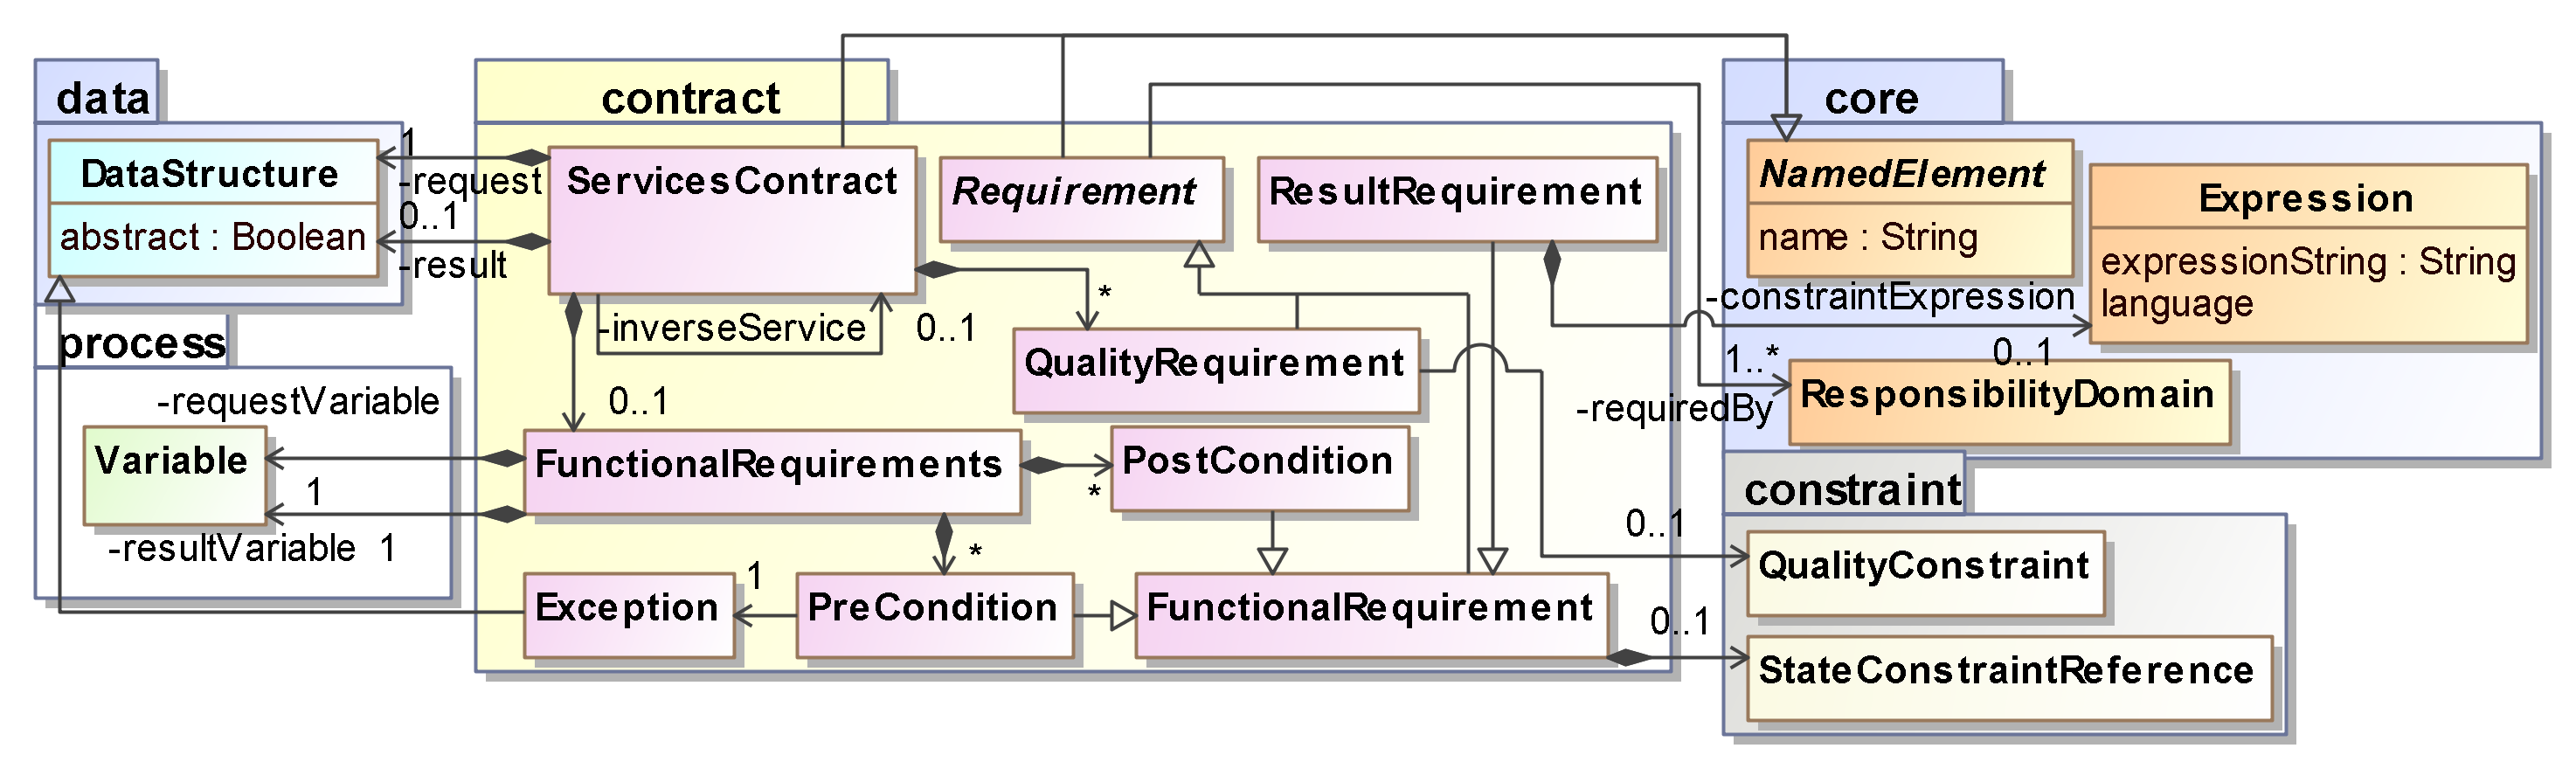
\includegraphics{contract}
  \caption{The modeling constructs available in URDAD introducing the semantics for services contracts}
  \label{fig:contractModule}
\end{figure}

We start by eliciting the stakeholders (yielding the stakeholders identified in section \ref{sec:qualityRequirements}) and their functional requirements. The output is a service contract specification for the \emph{performAnalysis} service which itself contains the concept of a service contract. The URDAD metamodel support for service contract specification is shown in figure \ref{fig:contractModule}. Below we use the text grammar defined for the URDAD-DSL to specify the service contract for the \emph{performAnalysis} service:

\lstset{language=urdad,caption=Specifying a state constraint in the URDAD text grammar.,label=contractTextSyntax}
\begin{lstlisting}[numbers=left,escapechar=|]
ResponsibilityDomain Analysis
{
  ...
  ServiceContract performAnalysis 
  {
    FunctionalRequirements receiving Variable performAnalysisRequest ofType PerformAnalysisRequest yielding Variable performAnalsysiResult ofType PerformAnalysisResult
    {
      PreCondition serviceHasStakeholders requiredBy (Client) raises NoStakeholdersException checks Constraint ServiceHasStakeholders with Query OCL:"performAnalaysisRequest.serviceRequirements"
      PreCondition stakeholderRequirementsConsistent requiredBy (Client Development Architecture Testing) raises InconsistentStakeholderRequirementsException checks Constraint StakeholderRequirementsConsistent with Query OCL:"performAnalysisResult.serviceContract"
      PostCondition serviceContractSpecified requiredBy (Client Development Architecture Testing) ensures Constraint ServiceContractSpecified with Query OCL:"performAnalysisResult"
      PostCondition serviceContractAssignedToResponsibilityDomain requiredBy (Client) ensures Constraint ServiceContractAssignedToResponsibilityDomain with Query OCL:"performAnalysisResult.serviceContract"
    }
    Request DataStructure PerformAnalysisRequest
    {
      has Component serviceRequirements ofType _ServiceRequirements
      has many Identification stakeholders identifying _Stakeholder
    }
    Result DataStructure PerformAnalysisResult
    {
      has Component serviceContract ofType _ServiceContract
    }
  }
}
\end{lstlisting}

Note how we are already regenerating the URDAD metamodel in that the \verb+ServiceContract+ for perform analysis generates a domain which includes the concept of a \verb+_ServiceContract+. As we follow the URDAD methodology to design itself, we traverse levels of granularity, incrementally generating lower level aspects of the URDAD process and the URDAD metamodel, populating the finer details in the metamodel classes and the lower level process elements of the URDAD process. Throughout the classes without underscore prefix are the metamodel classes whilst the classes with underscore prefix are the classes generated by the methodology itself. 

\lstset{language=urdad,caption=Regenerated metamodel classes.,label=constraintTextSyntax}
\begin{lstlisting}[numbers=left,escapechar=|]
DataStructure _ServiceContract 
{
    has Component functionalRequirements ofType _FunctionalRequirements
    has Component request ofType _DataStructure
    has Component result ofType _DataStructure
}
\end{lstlisting}

\begin{figure}[Htbp]
  \centering
  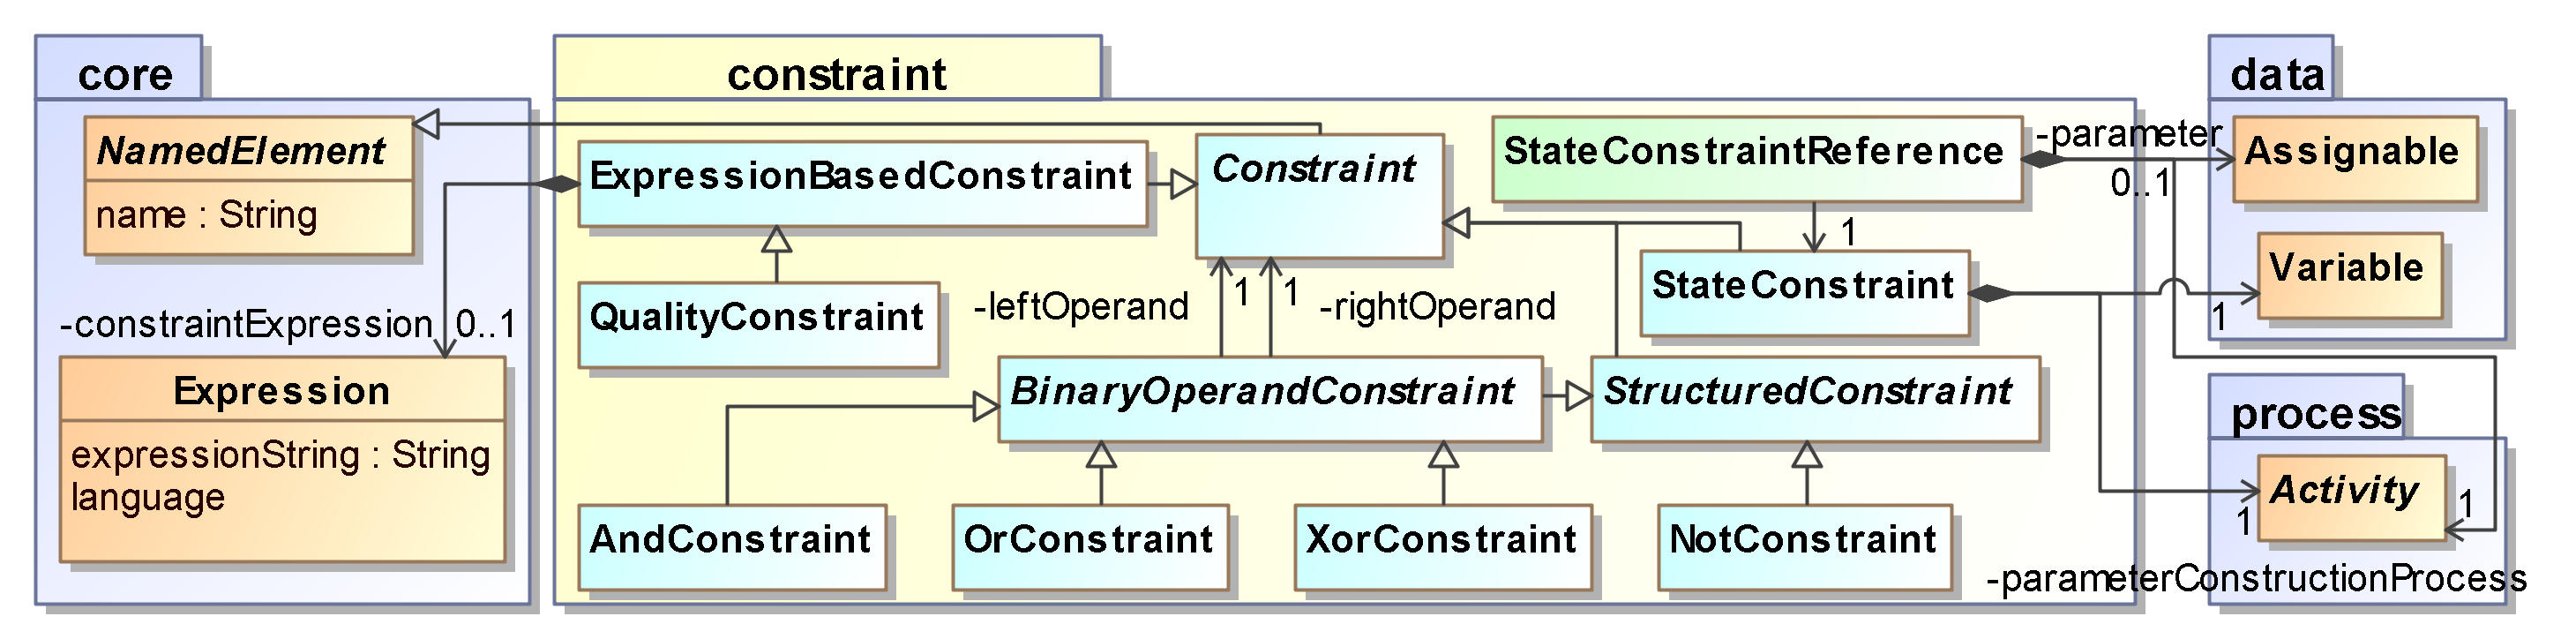
\includegraphics{constraint}
  \caption{The modeling constructs available in URDAD facilitating the specification of constraints.}
  \label{fig:constraintModule}
\end{figure}

Service contracts refers to reusable, parametrized state constraints. Figure \ref{fig:constraintModule}, shows URDAD's modeling elements for specifying such constraints. In a separate paper currently under review we have pointed out that the Object-Constraint Language (OCL)\cite{_object_2010}  alone is not expressive enough to specify reusable, parametrized constraints for a services oriented approach where one needs to extract information from the environment via services and then apply data structure constraints on the obtained environmental information.

The following listing shows an simple example of a parametrized constraint, \emph{ServiceHasStakeholders}, which demonstrated that a state constraint is assembled from a process that extracts information from the environment and a set of data constraints applied to the obtained information.
\lstset{language=urdad,caption=Specifying a state constraint in the URDAD text grammar.,label=processTextSyntax}
\begin{lstlisting}[numbers=left,escapechar=|]
StateConstraint ServiceHasStakeholders receiving Variable serviceRequirements ofType _ServiceRequirements 
{
  StateAssessmentProcess doSequential 
  {
    create Variable identifyStakeholdersRequest ofType IdentifyStakeholdersRequest
    set Query OCL:"identifyStakeholdersRequest.serviceRequirements" equalTo Query OCL:"serviceRequirements"
    requestService identifyStakeholders with identifyStakeholdersRequest yielding Variable identifyStakeholdersResult ofType IdentifyStakeholdersResult
  }
  Constraint OCL:"identifyStakeholdersResult->size() > 0"
}
\end{lstlisting}

\begin{figure}[Htbp]
  \centering
  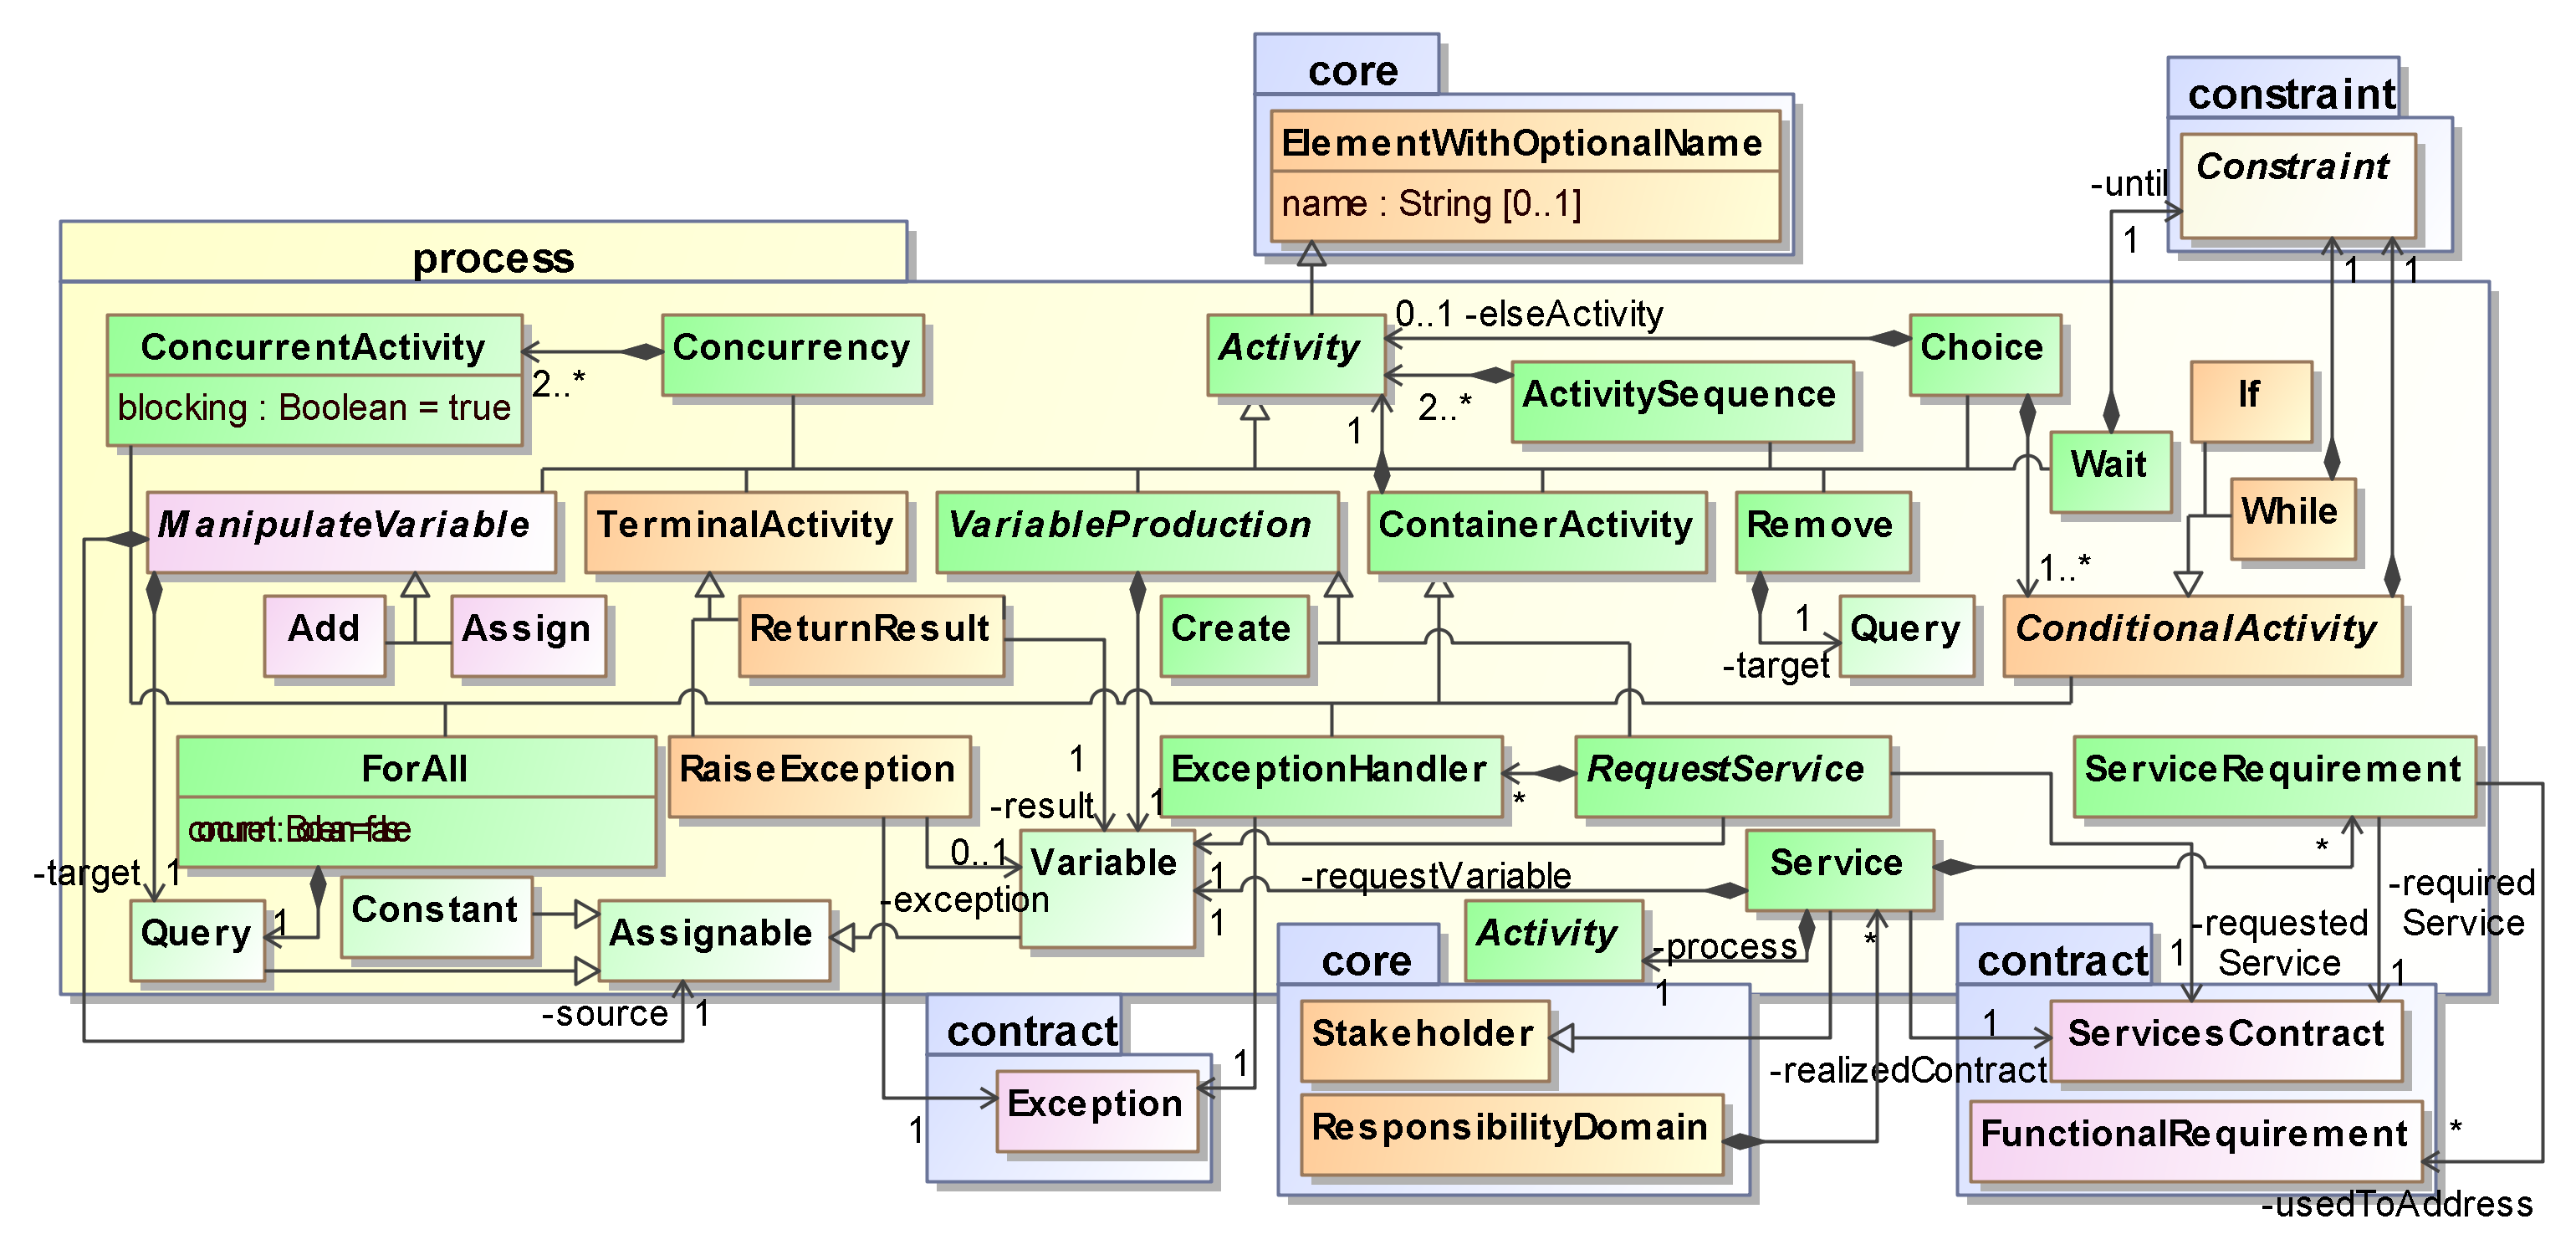
\includegraphics{process}
  \caption{The modeling constructs available for specifying services and processes in URDAD}
  \label{fig:processModule}
\end{figure}

Finally we use URDAD to design its analysis process. For this we use the URDAD modeling constructs for process specification shown in figure \ref{fig:processModule} (of course via the URDAD-DSL text grammar). Note that, following the URDAD process discussed in \ref{sec:urdadProcess} we first specify the services we want to use to address each of the functional requirements (the \verb+usedToAddress+ links between a service requirement and a functional requirement represents the satisfaction links of \cite{ramesh_toward_2001}) before choreographing the process across these services. 

The following listing is an excerpt of the URDAD analysis process generated by applying URDAD to design the \verb+performAnalysis+ service:
\lstset{language=urdad,caption=Specifying the performAnalysis service in the textual URDAD DSL syntax.,label=serviceTextSyntax}
\begin{lstlisting}[numbers=left,escapechar=|]
Service performAnalysisImpl realizes performAnalysis receiving Variable performAnalysisRequest ofType PerformAnalysisRequest 
{
  use identifyStakeholders toAddress (serviceHasStakeholders) 
  use specifyServiceContract toAddress (stakeholderRequirementsConsistent serviceContractSpecified)
  use assignServiceContractToResponsibilityDomain toAddress (serviceContractAssignedToResponsibilityDomain)
 
  Process doSequential
  {
    create Variable identifyStakeholdersRequest ofType IdentifyStakeholdersRequest
    set Query OCL:"identifyStakeholdersRequest.serviceRequirements" equalTo Query OCL:"performAnalysisRequest.serviceRequirements"
    
    requestService identifyStakeholders with identifyStakeholdersRequest yielding Variable identifyStakeholdersResult ofType IdentifyStakeholdersResult on NoStakeholdersException raiseException NoStakeholdersException

    ...
    requestService specifyServiceContract ...
    ...
    requestService assignServiceContractToResponsibilityDomain ...
    ...
    create Variable performAnalysisResult ofType PerformAnalysisResult
    set Query OCL:"performAnalysisResult.serviceContract" equalTo Query OCL:"specifyServiceContractResult.serviceContract"  
  }                              
}
\end{lstlisting}

Comparing the above listing we see that \emph{performAnalysis} process corresponds to the original process discussed in section \ref{secUrdadProcess}.